\documentclass[11pt]{article}

\usepackage{deauthor,times,graphicx}
\usepackage{wrapfig}
%\graphicspath{{Idreos/}}

\begin{document}

\title{Learning Data Structure Alchemy}

\author{
Stratos Idreos\quad
Kostas Zoumpatianos\quad
Subarna Chatterjee\quad
Wilson Qin\quad
Abdul Wasay\quad\\
Brian Hentschel\quad
Mike Kester\quad
Niv Dayan\quad
Demi Guo\quad
Minseo Kang\quad
Yiyou Sun\\\\
Harvard University
} 

 \maketitle 


 \begin{abstract}
 We propose a solution based on first principles and AI to the decades-old problem of data structure design. Instead of working on individual designs that each can only be helpful in a small set of environments, we propose the construction of an engine, a Data Alchemist, which learns how to blend fine-grained data structure design principles to automatically synthesize brand new data structures.
 \end{abstract}

\section{Computing Instead of Inventing Data Structures}

\begin{wrapfigure}[14]{r}{.4\textwidth}
\center
\vspace{-2.5em}
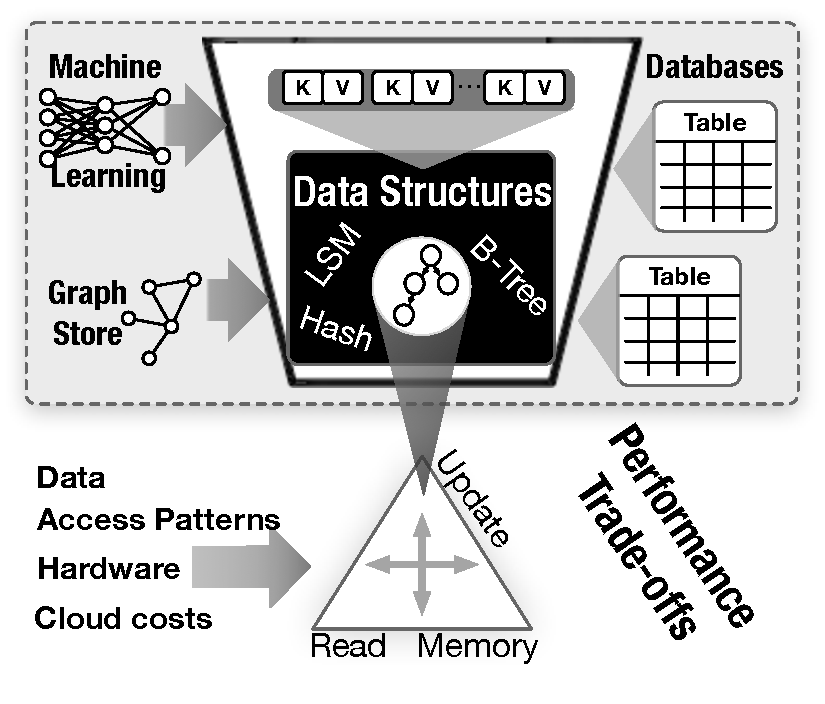
\includegraphics[width=.4\textwidth]{figs/IntroFigure.pdf}
\vspace{-3em}
\caption{Design trade-offs.}
\label{fig:rum}
\end{wrapfigure}What do analytics, machine learning, data science, and big data systems have in common? What is the major common component for astronomy, biology, neuroscience, and all other data-driven and computational sciences? Data structures. 

Data structures are one of the most fundamental areas of computer science. They are at the core of all subfields, including data systems, compilers, operating systems, human-computer interaction systems, networks, and machine learning. A data structure defines how data is physically stored. \textbf{For all algorithms that deal with data, their design starts by defining a data structure} that  minimizes computation and data movement \cite{Abadi2013, Athanassoulis2016, Hellerstein1995, Graefe2011, Kraska2018, Lehman1986, Yao1977, Yao1978, Dayan2016}. For example, we can only utilize an optimized sorted search algorithm if the data is sorted and if we can maintain it efficiently in such a state. 
%Data structures may also be referred to as ``data containers'' or ``access methods''.

\textbf{A Hard, Open, and Continuous Problem.} Since the early days of computer science dozens of new data structures are published every year. The pace has increased over the last decade, with 50-80 new data structures yearly according to data from DBLP \cite{dblp}. This is because of 1) the growth of data, 2) the increasing number of data-driven applications, 3) more fields moving to a computational paradigm where data collection, storage, and analysis become critical, and 4)~hardware changes that require a complete redesign of data structures and algorithms. Furthermore, for the past several decades, the hardware trend is that computation (e.g., CPUs, GPUs) becomes increasingly faster relative to data movement (e.g, memory, disks). This makes data structure design ever more critical as the way we store data dictates how much data an algorithm moves. 
  

\textbf{There Is No Perfect Data Structure Design.} Each design is a compromise among the fundamental trade-offs \cite{Athanassoulis2016}: read, update, and memory amplification. This is depicted visually in Figure \ref{fig:rum}. 
Read amplification is how much excess data an algorithm is forced to read; due to hardware properties such as page-based storage, even when reading a single data item, an algorithm has to load all items of the respective page. Write amplification is how much excess data an algorithm has to write; maintaining the structure of the data during updates typically causes additional writes. Memory amplification is how much excess data we have to store; any indexing that helps navigate the raw data is auxiliary data. Overall, this complex three-way tradeoff causes each design to be effective for only specific workloads \cite{Athanassoulis2016}. For example, a Log-Structured Merge-tree (LSM-tree) relies on batching and logging data without enforcing a global order. While this helps with writes, it hurts reads since now a single read query (might) have to search all LSM-tree levels.  Similarly, a sorted array enforces an organization in the data which favors reads but hurts writes, e.g., inserting a new item in a sorted (dense) array requires rewriting half the array on average. In this way, there is no universally good design. To get good performance, the design of a data structure has to be tailored to the data, queries, and hardware of the target application. 
 
\textbf{The Vast Design Space Slows Progress.}
The design of a data structure consists of 1) a data layout, and 2) algorithms that support basic operations (e.g., put, get, update). The data layout design itself may be further broken down into 1) the base data layout, and 2) an index  which helps navigate the data, i.e., the leaves of a B$^{+}$tree and its inner nodes, or the buckets of a hash table and the hash-map. We use the term data structure design throughout the proposal to refer to the overall design of the base data layout, indexing, and the algorithms together. A data structure can be as simple as an array or as arbitrarily complex as using sophisticated combinations of hashing, range and radix partitioning, careful data placement, and encodings. There are so many different ways to design a data structure and so many moving targets that it has become a notoriously hard problem; it takes several months even for experts to design and optimize a new structure. Most often, the initial data structure decisions for a data-intensive system remain intact; it is too complex to redesign a data structure, predict what its impact would be as workload and hardware change, implement it, and integrate it within a complex system or pipeline. Along the same lines, it is very hard to know when and why the core data structure within a complex system will ``break'', i.e., when performance will drop below an acceptable threshold. 


\textbf{The Problem In Sciences.} For data-driven fields without computer science expertise, these low-level choices are impossible to make. The only viable solution is using suboptimal off-the-shelf designs or hiring expensive experts. Data science pipelines in astronomy, biology, neuroscience, chemistry and other emerging data-driven scientific fields, exhibit exactly those characteristics \cite{Stonebraker2012, Stonebraker2013}. Recognizing these needs, new systems with novel storage schemes appear continuously for targeted problems \cite{Fernandez2018, Papadopoulos2016, SciDB2016, Seering2012, Xing2018} and exploratory workloads \cite{Kersten2011,Wasay2015,Idreos2013,Idreos2015}. However, given the vast design space (we provide more intuition on that later), the likelihood that a single off-the-shelf data structure fits an evolving and complex scientific scenario with unpredictable and exploratory access patterns, is extremely small. We include a relevant quote from Efthimios Kaxiras, Prof. of Pure and Applied Physics at Harvard University: \textit{``In chemistry and materials science, there exist a huge number of possible structures for a given chemical composition. Scientists are struggling to find ways to sort through these structures in an efficient way. The development of tailored database platforms would open great opportunities for new research in materials and molecular design.''}


\textbf{The Problem In Business}. For both established companies and data-driven startups, the complexity leads to a slow design process and has severe cost side-effects \cite{Bernstein1987a,Cheung2015}. Time to market is of extreme importance, so data structure design stops when a design ``is due'' and only rarely when it ``is ready''. We include a quote from Mark Callahan, a data systems architect with more than two decades of experience: \textit{``Getting a new data structure into production takes years. Assumptions made about the workload and hardware are likely to change. Decisions today are frequently based on expert opinions, and these experts are in short supply.''}

\textbf{The Problem In Clouds.} In today's cloud-based world even slightly sub-optimal designs, e.g., by 1\%, translate to a massive loss in energy utilization \cite{Kossman2018} for the cloud provider and cloud expenses for the user. This implies two trends. First, getting as close to the optimal design is as critical as ever. Second, the way a data structure design translates to cost needs to be embedded in the design process, i.e., being able to trade among read, write, and memory as the relative costs of these resources change. Furthermore, cost policies can vary significantly among cloud providers which implies that for the same data, queries, and hardware, the optimal data structure can be different across different cloud providers. In sciences, for universities and labs that maintain their own cluster and thus are affected by energy costs, or use cloud infrastructure and thus are affected by operating costs, it is critical to manage those costs.

\textbf{The Research Challenge.}
The long-term challenge is whether we can easily or even automatically find the optimal storage design for a given problem. This has been recognized as an open problem since the early days of computer science. In his seminal 1978 paper, Turing award winner Robert Tarjan includes this problem in his list of the five major challenges for the future (which also included $P$ vs. $NP$) \cite{Tarjan1978}: \textit{``Is there a calculus of data structures by which one can choose the appropriate data representation and techniques for a given problem?''}. This is exactly the problem we attack. We identify the source of the problem to be that \textbf{there is currently no good way to predict the performance impact} of new workloads, hardware, and data structure designs; we need a full implementation and extensive testing. Similarly, \textbf{there is no good way to enumerate the possible designs so we can choose among them}. We make three critical observations.
\vspace{-.5em}
\begin{enumerate}
	\item Each data structure design can be described as a set of design concepts. These are all low-level design decisions, such as using partitioning, pointers, or direct addressing.
	\vspace{-.5em}
	\item Each new data structure can be classified in two ways: it contains a) a new combination or tuning of existing design concepts, or b) at least one new design concept.
	\vspace{-.5em}
	\item By now the research community has invented so many fundamental design concepts that most new designs are combinations or tunings of existing concepts.
\end{enumerate}
\vspace{-.5em}
\emph{\textbf{Thesis:} If we knew the possible design space of data structures, i.e., the exhaustive set of fundamental design principles, and the performance properties we get when we synthesize them in arbitrary (valid) permutations, then we can create an engine that allows us to reason about every design, no matter how complex. The challenge then translates to being able to search the massive design space.}

\vspace{.5em} 

\begin{wrapfigure}{l}{.38\textwidth}
\vspace{-5ex}
\center
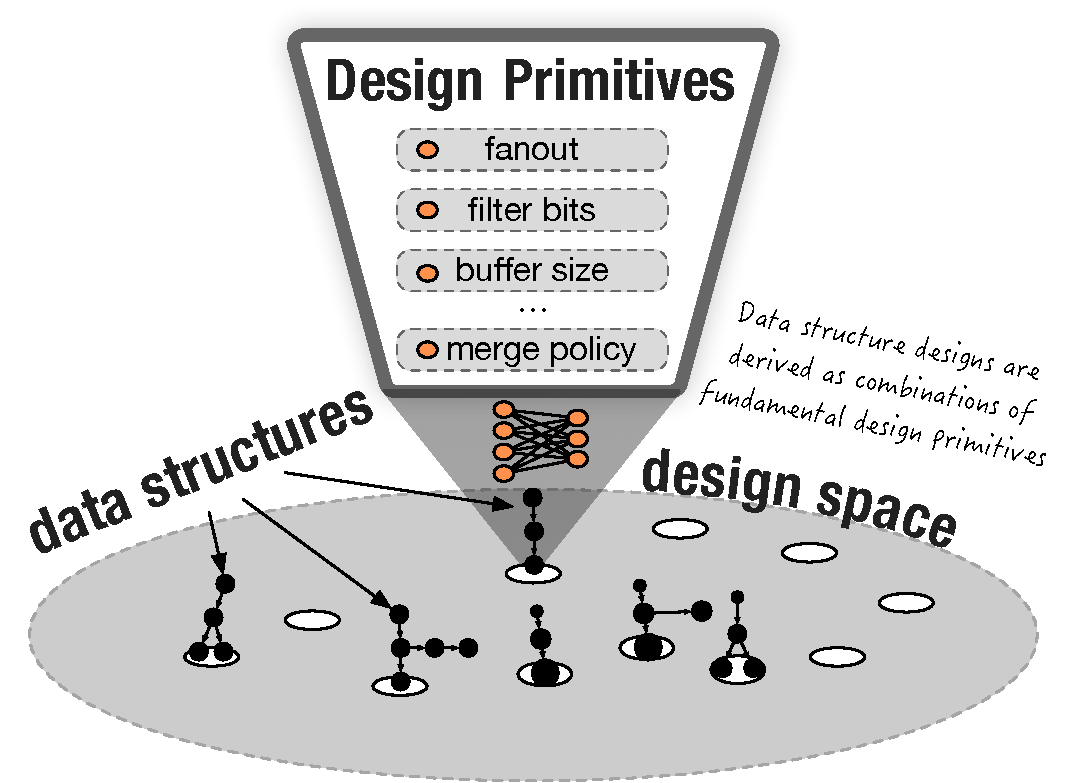
\includegraphics[width=.4\textwidth]{figs/IntroFigure2.pdf}
\vspace{-5ex}
\caption{Design from first principles.}
\vspace{-3ex}
\label{fig:concept}
\end{wrapfigure}
\textbf{Data Structure Alchemy.} We set out to discover the first principles of data structure design and develop algorithms to search through the massive design space they form. Our goal is to be able to reason about their combinations, tunings, and the performance properties they bring. Effectively, the principles and their structure form a ``grammar'' with which we can describe any data structure in a systematic way, including designs that have not been discovered yet. New designs can be ``calculated'' from the design space given constraints such as the expected workload, and hardware environment. If we focus on understanding and managing the core design elements, then new designs can be derived and existing designs can be transformed as if by magic - thus ``alchemy''.   

The vision and components of the engine we propose are captured in Figure \ref{fig:architecture}. We call this engine the Data Alchemist. Its functionality is to design a close-to-optimal data structure given a workload and hardware. The Data Alchemist takes four inputs: 1) the workload (queries and data) for which we would like to design an effective data structure, 2) a hardware profile where the data structure is expected to live, 3) optional performance and budget restrictions (e.g., point queries should be answered $\leq .3$ seconds), and 4) optional constraints for the search algorithms such as acceptable distance to the estimated optimal, a cap for the search time, and an initial design to bootstrap the search. 
%Optionally, a data structure specification can be given as input to be used as a starting point for the search and as a comparison point to the result. 
Then, the Data Alchemist outputs the resulting data structure design (abstract syntax tree) and its implementation in C\texttt{++} code. 

The architecture of the Data Alchemist gives us a clear path and methodology to make a dent in the decades-old problem of data structure design. Specifically, it boils down to the following contained challenges: 1) identifying the fundamental design principles, 2) creating methods that can estimate the behavior of full designs that blend more than one design primitives, and 3) creating practical search algorithms that utilize the previous two components and input constraints to generate designs automatically. In the rest of this paper, we summarize our existing work towards the first two goals and we focus on sketching the main research challenges and describe ideas on how to approach the goal of automated design. 

\section{Design Space and Cost Calculation via Model Synthesis.}

\textbf{Blending Design Principles.} The core idea is that the Data Alchemist contains a library of first principles which can be synthesized in arbitrary ways to give full data structure designs within a massive design space. We define the design of a data structure as the set of all decisions that characterize its data layout and algorithms, e.g., ``Should data nodes be sorted?'', ``Should they use pointers?'', and ``How should we scan them exactly?''. We define a first principle as a design concept that is not possible to break into more fine-grained concepts. For example, consider the design choice of linking two nodes of a data structure with a pointer. While there are potential tuning options (e.g., the size of the pointer), it is not possible to break this decision further; we either introduce a pointer or not. We separate design principles that have to do with the layout of a data structure from those that have to do with how we access the data. The bottom part of Figure \ref{fig:architecture} shows examples of data layout and access primitives for the key-value model.  Overall, a core part of our effort is in analyzing how fine-grained data structure principles behave in terms of critical performance metrics: read, write, concurrency, and storage size. We build models for those behaviors, and then develop methods that synthesize more complex data structure designs by putting together the models of multiple fine-grained design principles. 

We made a step toward towards this goal by introducing the \textbf{design space} of data structures supporting the key-value model \cite{Idreos2018}. The design space of data structures is defined by all designs that can be described as combinations and tunings of the ``first principles of data layout design''. As an analogy consider the periodic table of elements in~chemistry; it sketched the design space of existing elements based on their fundamental components, and allowed researchers to predict the existence of unknown, at the time, elements and their properties, purely by the structure of the design space. In the same way, we created the \textbf{periodic table of data structures} \cite{Idreos2018a} which describes more data structure designs than stars on the sky and can be used as a design discovery guide. 

Naturally, a design space does not necessarily describe ``all possible data structures''; a new design concept may be invented and cause an exponential increase in the number of possible designs. However, after 50 years of computer science research, the chances of inventing a fundamentally new design concept have decreased exponentially; many exciting innovations, in fact, come from utilizing a design concept that, while known, it was not explored in a given context before and thus it revolutionizes how to think about a problem. Using Bloom filters as a way to filter accesses in storage and remote machines, scheduling indexing construction actions lazily \cite{Idreos2007}, using ML models to guide data access \cite{Kraska2018}, storage \cite{Kersten2017} and other system components \cite{Kraska2019}, can all be thought of as such examples.
Design spaces that cover large fundamental sets of concepts can help accelerate progress with figuring out new promising directions, and when new concepts are invented they can help with figuring out the new possible derivative designs. For example, using models as part of the data structure design is an exciting recent idea, e.g., to replace the index layer or part of it \cite{Kraska2018,Kraska2019}. Such design options can become part of the design space for a more holistic design \cite{Idreos2019a}.

\begin{figure}[t]
    \center
  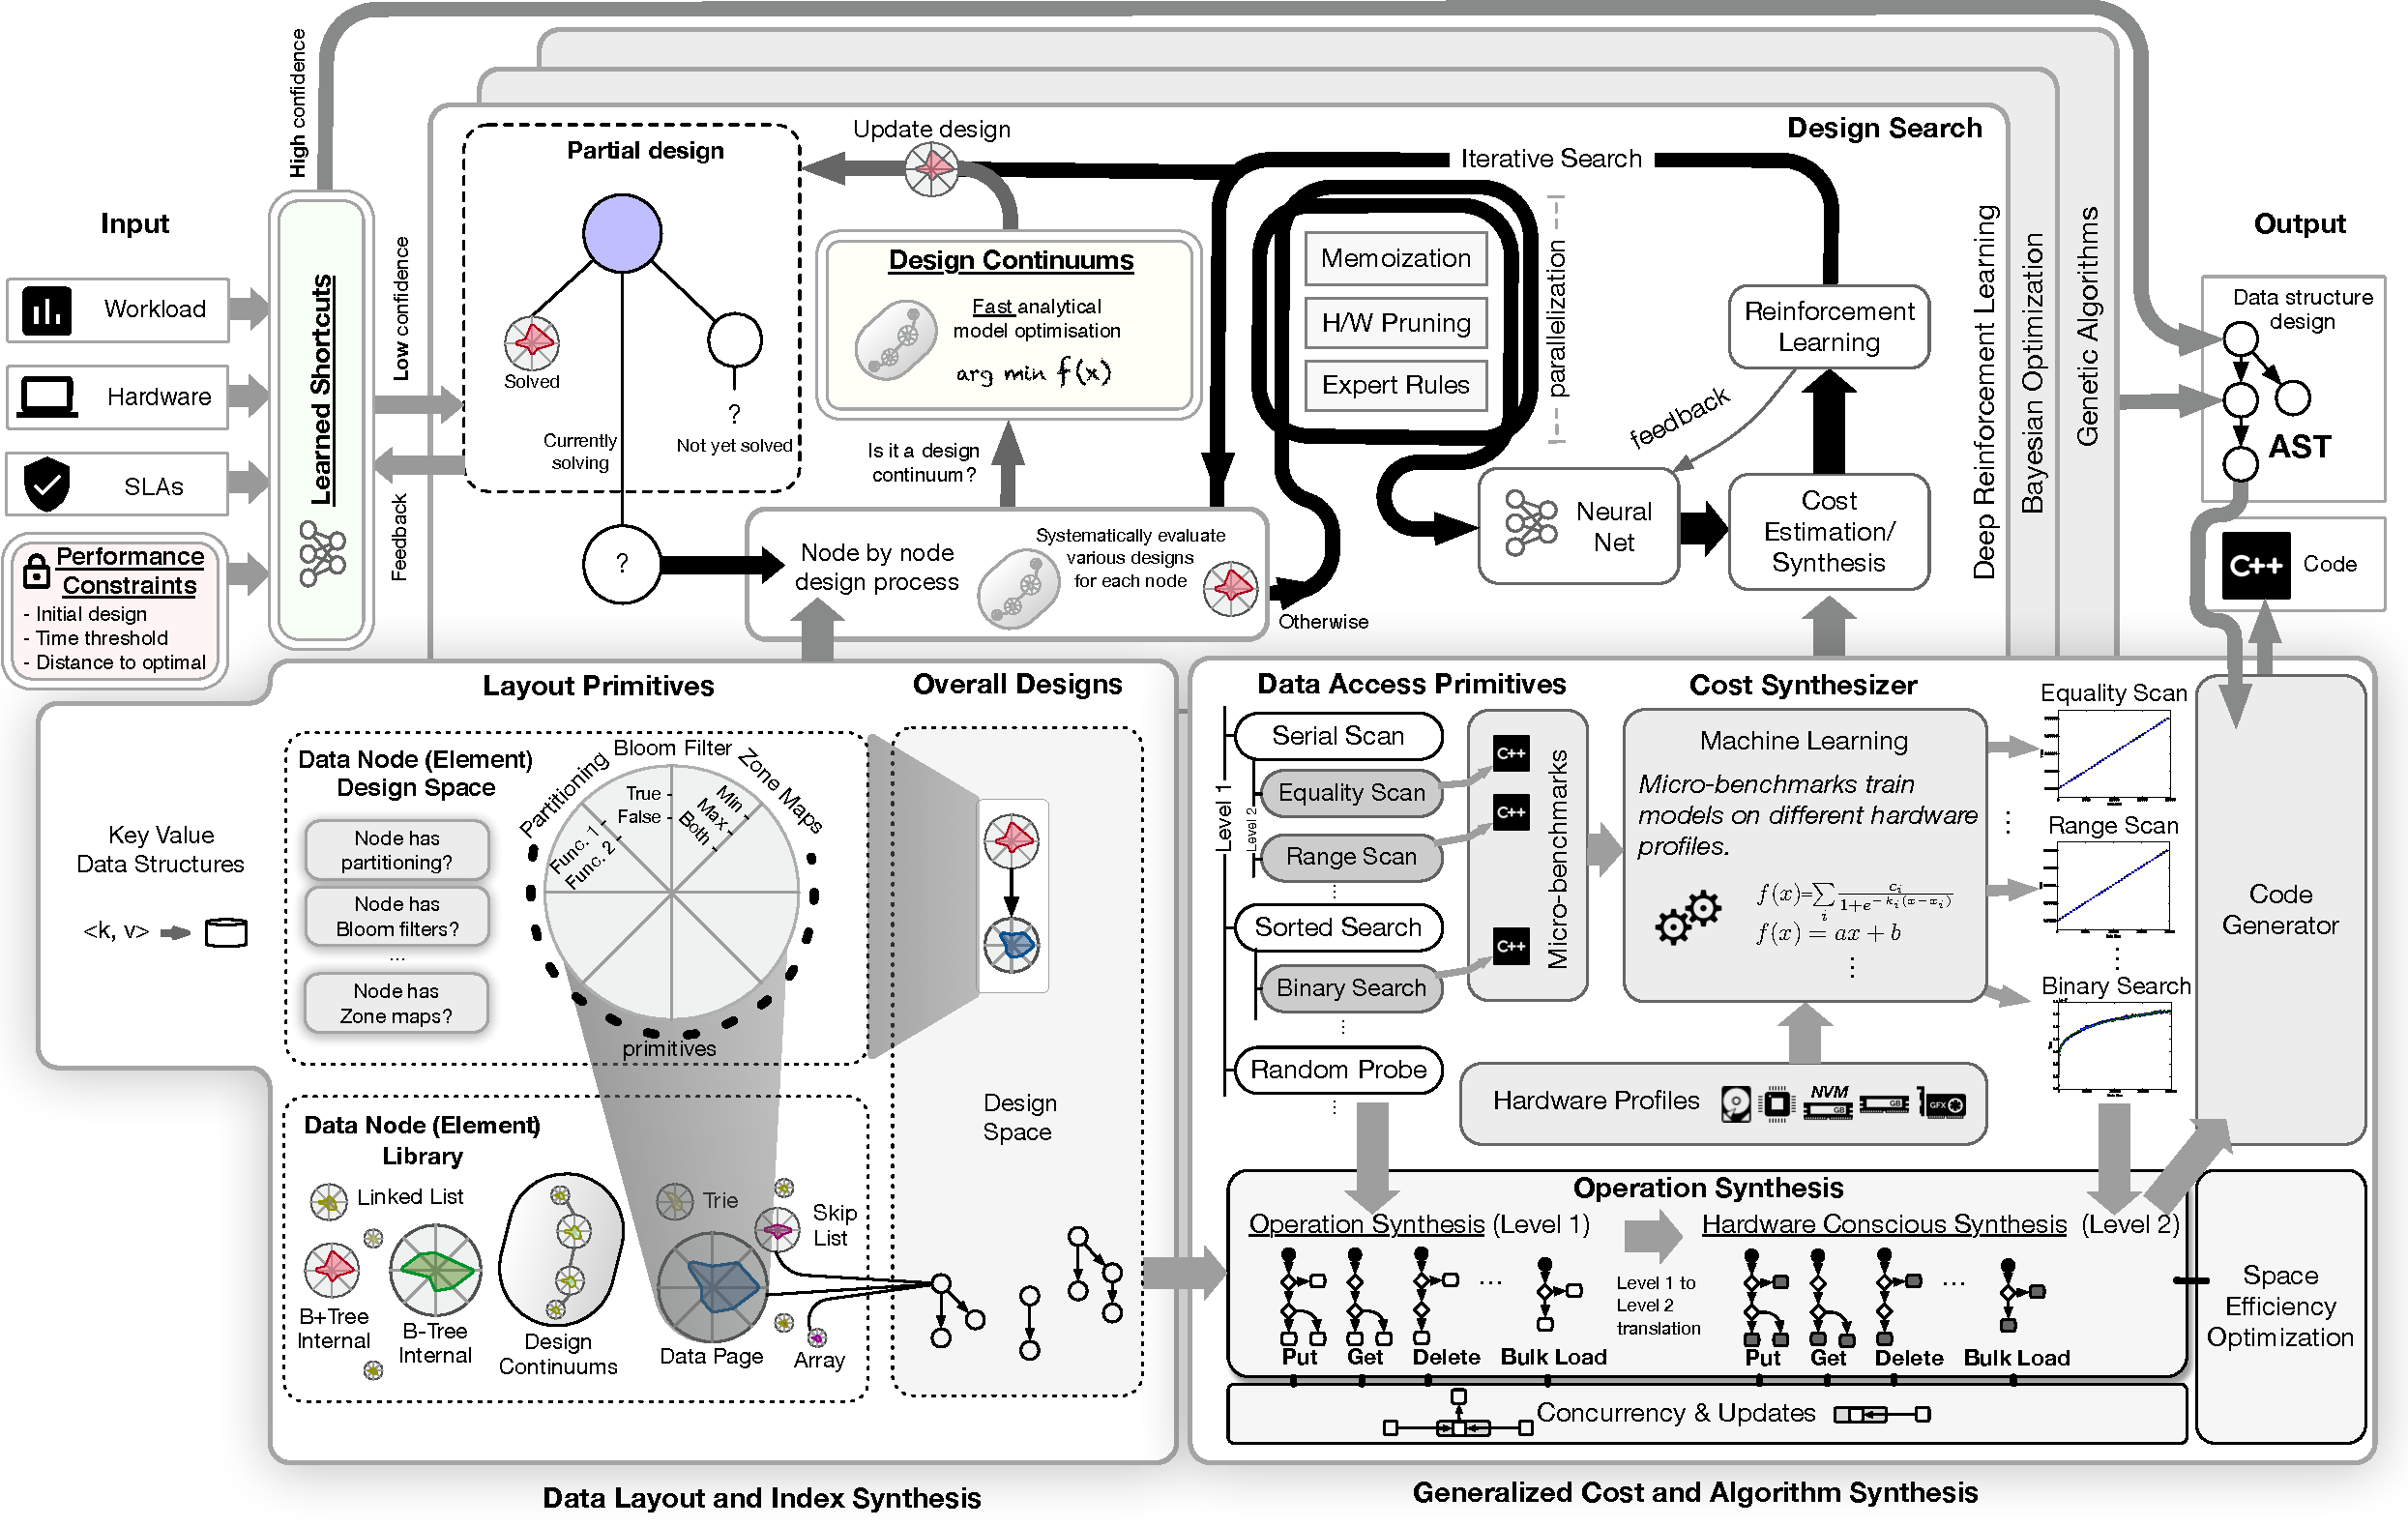
\includegraphics[width=\textwidth]{figs/Alchemy.pdf}
  \vspace{-6ex}
   \caption{The Data Alchemist architecture.}
   \vspace{-4ex}
   \label{fig:architecture}
\end{figure}

\textbf{Algorithm and Cost Synthesis from Learned Cost Models.}
To fully utilize the knowledge of the vast design space we need to be able to compare different designs in terms of expected performance. Complexity analysis explains how the properties of a design scale with data but does not give a precise performance computation given a workload and hardware. On the other hand, full implementation and testing on the target workload and hardware provide the exact performance. The combination of both complexity analysis and implementation gives the complete picture. The problem is that with so many designs possible in the design space, it is not feasible to analyze, implement, and test the numerous valid candidates. A less explored option is building generalized hardware-conscious cost models \cite{Manegold2002,Yao1977}. Similar to a full implementation, such models provide results very close to ground truth, and similar to complexity analysis they provide hints on how performance scales. However, building generalized models is nearly equally hard to a full implementation given the level of detail and hardware-conscious properties needed \cite{Kester2017}. In addition, any change in hardware properties requires retuning the model. Overall, arguing formally about the performance of diverse data structures designs, especially as workload and hardware properties change, is a notoriously hard problem \cite{Cardenas1973,Kester2017,Manegold2002,Teorey1976,Yao1977,Yao1975,Zhou1999}. In our case we want to perform this task for a massive number of candidate designs concurrently. 

We have shown that given a data structure definition that describes its layout, it is possible to automatically design the data access algorithms and compute their cost by \textbf{synthesizing operations from fundamental access primitives} on blocks of data \cite{Idreos2018,Idreos2018c}. There always exists a one-to-one mapping from a basic data layout to a high-level access pattern, e.g., if a data block is sorted we can utilize a sorted search. However, the performance that we would get out of a sorted search depends on 1)~the exact algorithm (binary search, interpolation search, etc.), 2) the specific hardware, and 3) the exact engineering (e.g., using a new set of SIMD instructions). The Data Alchemist will synthesize the detailed algorithm and compute the cost via a hybrid of analytical models, implementation, and machine learning. We call these \textbf{learned cost models}. For each generic class of access pattern (e.g., sorted search) on a block of data there exist many instances of algorithms and implementations. These are short implementations that capture the exact access pattern. For example, for a binary search, the implementation consists of an array of sorted integers where we perform a series of searches. During a training phase, this code runs on the desired hardware and we learn a model as data scales (across the memory hierarchy). Each model captures the subtle performance details of diverse hardware settings and the exact engineering used to build the code for each access pattern. To make training easier, our models start as analytical models since we know how these access patterns will likely behave. Using learned cost models, it is possible to compute the accurate performance even in the presence of skew, capturing caching effects and other hardware and workload properties \cite{Idreos2018,Idreos2018c}. The bottom right part of Figure \ref{fig:architecture} depicts examples of access principles and cost synthesis. 


\section{Learning to Design Data Structures}

Once we know what performance we get when we blend two or more design principles, then the next big challenge is to design algorithms that can try out different combinations to reach a good result in terms of performance (e.g., response time, storage space, budget). The design space, however, is not enough. The problem is that the design space is truly vast. For example, only for the key-value model \cite{Idreos2018,Idreos2018c} and without considering the extended design space needed for updates, concurrency control, and ML models, we estimate that the number of possible valid data structure designs explodes to $\gg10^{32}$ even if we limit the overall design to only two different kinds of nodes (e.g., as is the case for B$^{+}$tree). 

 Thus, it is hard even for experts to ``see'' the optimal solutions even if we give them the design space.  We need \textbf{search algorithms that navigate the possible design space to automatically design data structures} which are close to the best option (if not the best) given a desired workload and hardware. Using brute force and even dynamic programming variations leads to either impractical search times or we can only search through a small part of the design space. We study the properties of the design space as well as the properties of the applications using data structures to \textbf{turn the search process into a tractable problem in practice}. Our solutions lie in  machine learning based algorithms that utilize model synthesis, hardware-conscious termination triggers, expert knowledge to lead the search algorithms in the right direction, and when possible closed-form models to quickly search within sub-spaces of the larger space. Our agenda involves designing four components:

\begin{enumerate} 
	\item \textbf{Design Continuums} that allow us to search fast within pockets of the design space.
	\vspace{-.5em}
	\item \textbf{Performance Constraints} that provide application, user, and hardware based bounds. 
	\vspace{-.5em}
	\item \textbf{Learned Shortcuts} to accelerate a new search by learning from past results.
	\vspace{-.5em}
	\item \textbf{Practical Search Algorithms} that utilize continuums, constraints, and shortcuts.
\end{enumerate} 

 The overall search functionality is depicted at the top of Figure \ref{fig:architecture} and allows building and experimenting with many variations of search algorithms, constraints, and continuums. The high-level idea is that these algorithms treat the design space components of the Data Alchemist (bottom part of Figure \ref{fig:architecture}) as a black box to try out different combinations of design principles. For each combination, the estimated performance feeds into the search algorithm's policy. Next we describe each one of four components in more detail to discuss the vision and preliminary results. 

\textbf{Design Continuums.}
A key ingredient in any algorithm is to induce domain-specific knowledge. Our insight is that there exist ``design continuums''  in the design space of data structures which can accelerate the search algorithms. An intuitive way to think of design continuums is as a performance hyperplane that connects a subset of data structure designs. It can be thought of as a super-structure that encapsulates all those designs by taking advantage of the notion that those designs are synthesized from the same set of fundamental principles. 

A design continuum contains a set of rules to instantiate each one of its members and crucially a cost model with a single closed-form equation for each one of the core performance metrics (read, write, memory size) which applies across all member designs. In turn, closed-form models can be computed instantly to reason about this part of the design space. Thus we can search that part of the design space quickly to augment the search algorithms. 

We introduced the first design continuum that connects a set of key-value structures \cite{Idreos2019}. Specifically, we have shown that it is possible to connect diverse designs including Tiered LSM-tree \cite{Jagadish1997, Dayan2017, Dayan2018a, Dayan2019, Lakshman2010}, Lazy Leveled LSM-tree \cite{Dayan2018}, Leveled LSM-tree \cite{ONeil1996, Dayan2017, FacebookRocksDB, GoogleLevelDB}, COLA \cite{Bender2007, Jermaine2007}, FD-tree \cite{Li2010}, B$^{\epsilon}$tree \cite{Brodal2003, Arge2003, Bender2007, Jannen2015, Jermaine2007, Papagiannis2016}, and B$^{+}$tree \cite{Bayer1970}. 

Our goal is to discover and formalize as many design continuums as possible and connect them to our search algorithms such that when a search algorithm ``hits'' a continuum, it can instantaneously get the best design within that space using the closed-form models as shown at the top part of Figure \ref{fig:architecture}. One of the most exciting challenges here is to formalize design continuums that are based as much as possible on average case analysis as opposed to worst case as in \cite{Idreos2019}. This requires building unifying models that take into account properties such as data and query distribution as well as the state of the target data structure in a workload that contains a sequence of steps. 

Additional opportunities in creating ``searchable'' pockets of the design space include the use of integer solvers. This is for small parts of the design space which are potentially hard to formalize in a continuum but can be modeled as an integer problem. For example, consider partitioning of an array for optimal performance of a mix of point read, range read, update, delete, and insert operations. This is a small space that needs to be navigated by most data structures which contain blocks of data and partitioning can be a good option for each block. Each operation benefits or is hurt by partitioning in a different way, and so finding the right layout depending on the workload is a delicate balance. This problem can be mapped as a binary integer optimization problem and assigned directly to an integer solver. The Data Alchemist may contain numerous ``searchable pockets'' in the design space each one relying either on closed-form formulas or integer solvers.   

\textbf{Performance Constraints.} 
The larger the number of continuums we manage to create, the more tractable the search process becomes. However, due to the complexity of the design space, we expect that we will be able to generate many small continuums rather than few big ones (in terms of the number of designs they contain). As such, given the astronomical size of the design space, search algorithms will intuitively still have a massive number of candidates to consider. To provide the next level of speed-up we are working towards performance constraints that  bound search algorithms based on application, hardware and user context. 

First, we observe that \textbf{the ultimate possible performance is limited by the underlying hardware} in any given scenario. For example, if an application or a researcher/engineer enter a query to the Data Alchemist to find a good data structure design on hardware $H$, then immediately we can consult the learned models which were trained on $H$ for the best read, and write performance possible, e.g., reading or writing a single page from disk for a point read or write. Once a search algorithm finds a design within $k\%$ of these hardware imposed bounds, it can stop trying to improve as no further substantial improvements are possible. Parameter $k\%$ can be exposed as input as it is an application/user level decision. 

Another performance constraint is to use a data structure design (full or partial) that the user suggests as starting point. This allows to induce expert and application knowledge in the search algorithm. The search process then can \textbf{auto-complete} the design without having to reconsider the initial decisions (this feature can also be used to detect a ``bad'' original design). Other examples of constraints include a time bound on the overall time a search algorithm should run, i.e., returning a best effort result once this time passes as well as returning top-k results which includes classes of promising design decisions it did not have time to consider. The top left and central part of Figure \ref{fig:architecture} shows examples of constraints and how they can be used as part of a search algorithm to accelerate the search. 
 

\textbf{Learned Shortcuts.}
Another critical component to speed up the search algorithms is learning from past results. We design and employ diverse neural network ensamples which are fed by an embedding generated using the input query, data, and hardware of every request and then it is ``labeled'' by the resulting output data structure design. Our goal is to create shortcuts through supervised learning that can practically instantly answer future queries without going through the search process, or alternatively the output of the neural network can work as a good starting point for a search. The top left part of Figure \ref{fig:architecture} shows how this fits in a search algorithm. Our work also includes accelerating the training and inference of neural network ensamples to achieve interactive speed and quick reaction to new workloads \cite{Wasay2018}.

\textbf{Algorithms.} We design black box optimization algorithms that utilize continuums, constraints, and shortcuts to find a good design as fast as possible given a request.  This includes Genetic Algorithms (GA) \cite{Idreos2017}, Bayesian Optimization (BO), and Deep Reinforcement Learning (DRL). There are numerous challenges. For example, let us consider reinforcement learning. First, we must formalize the space of actions and rewards in data structure design. We experiment with both policy-based approaches that design the entire data structure at a time, and action-based approaches that design individual nodes at a time as well as hybrids. One approach is to model the design of a data structure as a multi-armed bandit problem. That is, we have a design space of design decisions that can be synthesized to a massive number of ``design elements'' as shown in Figure \ref{fig:architecture}. Each element can be seen as a bandit that can be chosen for any node of a data structure. Then, the problem is bounded by the number of different types of nodes we would like to include in the final data structure design. For example, the majority of the published key-value data structures consist of two node types, the index and the data, with Masstree \cite{Mao2012} and Bounded Disorder \cite{Litwin1986} being exceptions that consist of three types of node. With the Data Alchemist we have the opportunity to explore designs with an arbitrary number of node types.


We expect that \textbf{no single algorithm will be a universal solution}. This is because of the core principles of how these families of algorithms behave in terms of convergence and response time. In the case of GA, exploration happens through mutation, exploitation is a result of the crossover and the selection process, whereas history is maintained implicitly through the surviving population. When it comes to BO, exploration happens by selecting solutions with high variance (i.e., solutions we are less certain about), exploitation, on the other hand, happens through selecting solutions with high mean (i.e., solutions we are quite sure about). History is maintained by a combination of the acquisition function and the probabilistic model. Finally, DRL makes conditional choices to explore the solution space, picks solutions with a high expected reward to exploit existing knowledge, and history is maintained in a deep neural network. As such, they all behave differently depending on the complexity of the problem at hand, desired span of the search through the design space, convergence speed, and the desired  properties of the resulting data structure design (robustness vs. ultimate performance). The Data Alchemist  incorporates several algorithms as shown at the top part of Figure \ref{fig:architecture} and choose the right one depending on the context. 
%For instance, BO is efficient in terms of the number of various solutions it tries. This is because when exploring, BO explicitly picks solutions that minimize the overall uncertainty in the solution space. On the flip side, BO is conservative and may not try out as many random solutions. DRL, as opposed to this, tries out a configurable proportion of completely random solutions and in highly complex solution spaces may result in better solutions. DRL, however, requires more computational resources to learn as it has to update a deep neural network. Finally, GA provides two distinct advantages: (i) It leverages parallelism by trying out multiple solutions in every iteration, and (ii) It moves slowly through the solution space providing more robust intermediate solutions before it converges to a final solution. This may take more time to converge to the ultimate solution.

\textbf{Learned Models for Complex Patterns.}
The Data Alchemist constructs the cost of data structure designs out of fine-grained primitives for which it knows learned models. However, a complex design inevitably loses accuracy when synthesized out of many models. A solution is to generate the code for sets of design primitives and learn a single compound model for all of them via on-the-fly experiments during the search algorithm (there are too many possible compound models to train for all of them a priori). Results can also be cached in the learned models library for future use. Such compound models can increase the accuracy of the search algorithms, leading to better data structure designs. We build a compiler to generate this code by directly utilizing the fact that we already have the code of the individual learned models in the library. This compiler can also be used to output starter code for the resulting design of a search using the abstract syntax tree of the design and the code of the learned models that were chosen by the search algorithm. This makes it easier to adopt, extend, and fine-tune designs. 

\section{Inspiration}
Our work is inspired by numerous efforts that also use first principles and clean abstractions to understand a complex design space. John Ousterhout's project Magic allows for quick verification of transistor designs so that engineers can easily test multiple designs synthesized by basic concepts \cite{Ousterhout1984}. Leland Wilkinson's ``grammar of graphics'' provides structure and formulation on the massive universe of possible graphics \cite{Wilkinson2005}. Timothy G. Mattson's work creates a language of design patterns for parallel algorithms \cite{Mattson2004}. Mike Franklin's Ph.D. thesis explores the possible client-server architecture designs using caching based replication as the main design primitive \cite{Franklin1993}. 
Joe Hellerstein's work on Generalized Search Trees makes it easy to design and test new data structures by providing templates which expose only a few options where designs need to differ \cite{Hellerstein1995,Aoki1998,Aoki1999,Kornacker1997,Kornacker1999,Kornacker1998,Kornacker2003}. 
S. Bing Yao's \cite{Yao1977} and 
Stefan Manegold's \cite{Manegold2002} work on generalized hardware conscious cost models showed that it is possible to synthesize the costs of complex operations from basic access patterns. 
Work on data representation synthesis in programming languages enables synthesis of representations out of small sets of (3-5) existing data structures \cite{Schonberg1979,Schonberg1981,Cohen1993,Smaragdakis1997,Shacham2009,Hawkins2011,Hawkins2012,Loncaric2016,Steindorfer2016}. 
Work on tuning \cite{Ioannidis1987, Chaudhuri1997} and adaptive systems is also relevant as conceptually any adaptive technique tunes along part of the design space. For example, work on hybrid data layouts and adaptive indexing automates selection of the right layout \cite{Arulraj2016,Alagiannis2014, Hankins2003,Idreos2007,Dittrich2011,Schuhknecht2013,Alvarez2014, Liu2016, Dayan2017, Pirk2014, Graefe2012a,Petraki2015,Zoumpatianos2014,Idreos2009, Kennedy2015,Sleator1985}. Similarly works on tuning via experiments \cite{Babu2009}, learning \cite{Anderson2013}, and tuning via machine learning \cite{Aken2017,Heimel2015} can adapt parts of a design using feedback from tests.

\section{Summary and Future Steps}
We describe the path toward automating data structure invention and design from first principles and AI. The secret sauce is in finding the first principles of design, mapping the design space that they form, being able to reason about the expected performance of designs, and finally building practical AI algorithms that can navigate this space to design new data structures. Searching the whole massive space is not likely possible so the key is in translating as much design and application knowledge into the search algorithms. Our ongoing efforts include applying this same methodology of first principles and AI beyond traditional key-value structures, focusing on forming the design space of statistics computation \cite{Wasay2017}, neural networks \cite{Wasay2018}, and sketches \cite{Hentschel2018}.

% \begin{small}
% \bibliographystyle{abbrv}
% \bibliography{../das/Bibliography-Mendeley/library,../das/Bibliography-Mendeley/to-be-added}
 \begin{thebibliography}{10} 
 \itemsep=1pt 
 \begin{small}

\bibitem{Abadi2013}
D.~J. Abadi, P.~A. Boncz, S.~Harizopoulos, S.~Idreos, and S.~Madden.
\newblock {The Design and Implementation of Modern Column-Oriented Database
  Systems}.
\newblock {\em Foundations and Trends in Databases}, 5(3):197--280, 2013.

\bibitem{Aken2017}
D.~V. Aken, A.~Pavlo, G.~J. Gordon, and B.~Zhang.
\newblock {Automatic Database Management System Tuning Through Large-scale
  Machine Learning}.
\newblock ACM SIGMOD, 2017.

\bibitem{Alagiannis2014}
I.~Alagiannis, S.~Idreos, and A.~Ailamaki.
\newblock {H2O: A Hands-free Adaptive Store}.
\newblock ACM SIGMOD, 2014.

\bibitem{Alvarez2014}
V.~Alvarez, F.~M. Schuhknecht, J.~Dittrich, and S.~Richter.
\newblock {Main Memory Adaptive Indexing for Multi-Core Systems}.
\newblock DAMON, 2014.

\bibitem{Anderson2013}
M.~R. Anderson, D.~Antenucci, V.~Bittorf, M.~Burgess, M.~J. Cafarella,
  A.~Kumar, F.~Niu, Y.~Park, C.~R{\'{e}}, and C.~Zhang.
\newblock {Brainwash: A Data System for Feature Engineering}.
\newblock CIDR, 2013.

\bibitem{Aoki1998}
P.~M. Aoki.
\newblock {Generalizing "Search" in Generalized Search Trees (Extended
  Abstract)}.
\newblock IEEE ICDE, 1998.

\bibitem{Aoki1999}
P.~M. Aoki.
\newblock {How to Avoid Building DataBlades That Know the Value of Everything
  and the Cost of Nothing}.
\newblock SSDBM, 1999.

\bibitem{Arge2003}
L.~Arge.
\newblock {The Buffer Tree: A Technique for Designing Batched External Data
  Structures}.
\newblock {\em Algorithmica}, 2003.

\bibitem{Arulraj2016}
J.~Arulraj, A.~Pavlo, and P.~Menon.
\newblock {Bridging the Archipelago between Row-Stores and Column-Stores for
  Hybrid Workloads}.
\newblock ACM SIGMOD, 2016.

\bibitem{Athanassoulis2016}
M.~Athanassoulis, M.~S. Kester, L.~M. Maas, R.~Stoica, S.~Idreos, A.~Ailamaki,
  and M.~Callaghan.
\newblock {Designing Access Methods: The RUM Conjecture}.
\newblock EDBT, 2016.

\bibitem{Babu2009}
S.~Babu, N.~Borisov, S.~Duan, H.~Herodotou, and V.~Thummala.
\newblock {Automated Experiment-Driven Management of (Database) Systems}.
\newblock HotOS, 2009.

\bibitem{Bayer1970}
R.~Bayer and E.~M. McCreight.
\newblock {Organization and Maintenance of Large Ordered Indexes}.
\newblock ACM SIGFIDET Workshop on Data Description
  and Access, 1970.

\bibitem{Bender2007}
M.~A. Bender, M.~Farach-Colton, J.~T. Fineman, Y.~R. Fogel, B.~C. Kuszmaul, and
  J.~Nelson.
\newblock {Cache-Oblivious Streaming B-trees}.
\newblock SPAA, 2007.

\bibitem{Bernstein1987a}
P.~A. Bernstein and D.~B. Lomet.
\newblock {CASE Requirements for Extensible Database Systems}.
\newblock {\em IEEE Data Engineering Bulletin}, 10(2):2--9, 1987.

\bibitem{Brodal2003}
G.~S. Brodal and R.~Fagerberg.
\newblock {Lower Bounds for External Memory Dictionaries}.
\newblock SODA, 2003.

\bibitem{Cardenas1973}
A.~F. Cardenas.
\newblock {Evaluation and Selection of File Organization - a Model and System}.
\newblock {\em Communications of the ACM}, (9):540--548, 1973.

\bibitem{Chaudhuri1997}
S.~Chaudhuri, V.~R. Narasayya.
\newblock {An Efficient Cost-Driven Index Selection Tool for Microsoft SQL
  Server}.
\newblock VLDB'97.

\bibitem{Cheung2015}
A.~Cheung.
\newblock {Towards Generating Application-Specific Data Management Systems}.
\newblock CIDR, 2015.

\bibitem{Cohen1993}
D.~Cohen and N.~Campbell.
\newblock {Automating Relational Operations on Data Structures}.
\newblock {\em IEEE Software}, 1993.

\bibitem{Dayan2017}
N.~Dayan, M.~Athanassoulis, and S.~Idreos.
\newblock {Monkey: Optimal Navigable Key-Value Store}.
\newblock ACM SIGMOD, 2017.

\bibitem{Dayan2018a}
N.~Dayan, M.~Athanassoulis, S.~Idreos.
\newblock {Optimal Bloom Filters and Adaptive Merging for LSM-Trees}.
\newblock TODS'18.

\bibitem{Dayan2016}
N.~Dayan, P.~Bonnet, and S.~Idreos.
\newblock {GeckoFTL: Scalable Flash Translation Techniques For Very Large Flash
  Devices}.
\newblock ACM SIGMOD, 2016.

\bibitem{Dayan2018}
N.~Dayan and S.~Idreos.
\newblock {Dostoevsky: Better Space-Time Trade-Offs for LSM-Tree Based
  Key-Value Stores via Adaptive Removal of Superfluous Merging}.
\newblock ACM SIGMOD, 2018.

\bibitem{Dayan2019}
N.~Dayan and S.~Idreos.
\newblock The log-structured merge-bush \& the wacky continuum.
\newblock ACM SIGMOD, 2019.

\bibitem{dblp}
DBLP.
\newblock {Computer Science Bibliography}.
\newblock {\em https://dblp.uni-trier.de}, 2019.

\bibitem{Dittrich2011}
J.~Dittrich and A.~Jindal.
\newblock {Towards a One Size Fits All Database Architecture}.
\newblock CIDR, 2011.

\bibitem{FacebookRocksDB}
Facebook.
\newblock {RocksDB}.
\newblock {\em https://github.com/facebook/rocksdb}.

\bibitem{Fernandez2018}
R.~C. Fernandez, Z.~Abedjan, F.~Koko, G.~Yuan, S.~Madden, and M.~Stonebraker.
\newblock Aurum: {A} data discovery system.
\newblock IEEE ICDE, 2018.

\bibitem{Franklin1993}
M.~J. Franklin.
\newblock {\em {Caching and Memory Management in Client-Server Database
  Systems}}.
\newblock PhD thesis, University of Wisconsin-Madison, 1993.

\bibitem{GoogleLevelDB}
Google.
\newblock {LevelDB}.
\newblock {\em https://github.com/google/leveldb/}.

\bibitem{Graefe2011}
G.~Graefe.
\newblock {Modern B-Tree Techniques}.
\newblock {\em Foundations and Trends in Databases}, 3(4):203--402, 2011.

\bibitem{Graefe2012a}
G.~Graefe, F.~Halim, S.~Idreos, H.~Kuno, S.~Manegold.
\newblock {Concurrency control for adaptive indexing}.
\newblock PVLDB'12.

\bibitem{Hankins2003}
R.~A. Hankins and J.~M. Patel.
\newblock {Data Morphing: An Adaptive, Cache-Conscious Storage Technique}.
\newblock VLDB, 2003.

\bibitem{Hawkins2012}
P.~Hawkins, A.~Aiken, K.~Fisher, M.~C. Rinard, and M.~Sagiv.
\newblock {Concurrent data representation synthesis}.
\newblock PLDI, 2011.

\bibitem{Hawkins2011}
P.~Hawkins, A.~Aiken, K.~Fisher, M.~C. Rinard, and M.~Sagiv.
\newblock {Data Representation Synthesis}.
\newblock PLDI, 2011.

\bibitem{Heimel2015}
M.~Heimel, M.~Kiefer, and V.~Markl.
\newblock {Self-Tuning, GPU-Accelerated Kernel Density Models for
  Multidimensional Selectivity Estimation}.
\newblock ACM SIGMOD, 2015.

\bibitem{Hellerstein1995}
J.~M. Hellerstein, J.~F. Naughton, and A.~Pfeffer.
\newblock {Generalized Search Trees for Database Systems}.
\newblock VLDB, 1995.

\bibitem{Hentschel2018}
B.~Hentschel, M.~S. Kester, and S.~Idreos.
\newblock {Column Sketches: A Scan Accelerator for Rapid and Robust Predicate
  Evaluation}.
\newblock ACM SIGMOD, 2018.

\bibitem{Idreos2013}
S.~Idreos.
\newblock {Big Data Exploration}.
\newblock In {\em Big Data Computing}. Taylor and Francis, 2013.

\bibitem{Idreos2019}
S.~Idreos, N.~Dayan, W.~Qin, M.~Akmanalp, S.~Hilgard, A.~Ross, J.~Lennon,
  V.~Jain, H.~Gupta, D.~Li, and Z.~Zhu.
\newblock Design continuums and the path toward self-designing key-value stores
  that know and learn.
\newblock CIDR, 2019.

\bibitem{Idreos2007}
S.~Idreos, M.~L. Kersten, and S.~Manegold.
\newblock {Database Cracking}.
\newblock CIDR, 2007.

\bibitem{Idreos2009}
S.~Idreos, M.~L. Kersten, S.~Manegold.
\newblock {Self-organizing Tuple Reconstruction in Column-Stores}.
\newblock ACM SIGMOD'09.

\bibitem{Idreos2019a}
S.~Idreos and T.~Kraska.
\newblock From auto-tuning one size fits all to self-designed and learned
  data-intensive systems.
\newblock ACM SIGMOD, 2019.

\bibitem{Idreos2017}
S.~Idreos, L.~M. Maas, and M.~S. Kester.
\newblock {Evolutionary Data Systems}.
\newblock {\em CoRR}, abs/1706.0, 2017.

\bibitem{Idreos2015}
S.~Idreos, O.~Papaemmanouil, and S.~Chaudhuri.
\newblock {Overview of Data Exploration Techniques}.
\newblock ACM SIGMOD, 2015.

\bibitem{Idreos2018a}
S.~Idreos, K.~Zoumpatianos, M.~Athanassoulis, N.~Dayan, B.~Hentschel, M.~S.
  Kester, D.~Guo, L.~M. Maas, W.~Qin, A.~Wasay, and Y.~Sun.
\newblock {The Periodic Table of Data Structures}.
\newblock {\em IEEE Data Engineering Bulletin}, 41(3):64--75, 2018.

\bibitem{Idreos2018}
S.~Idreos, K.~Zoumpatianos, B.~Hentschel, M.~S. Kester, and D.~Guo.
\newblock {The Data Calculator: Data Structure Design and Cost Synthesis from
  First Principles and Learned Cost Models}.
\newblock ACM SIGMOD, 2018.

\bibitem{Idreos2018c}
S.~Idreos, K.~Zoumpatianos, B.~Hentschel, M.~S. Kester, and D.~Guo.
\newblock {The Internals of The Data Calculator}.
\newblock {\em CoRR}, abs/1808.02066, 2018.

\bibitem{Ioannidis1987}
Y.~E. Ioannidis and E.~Wong.
\newblock {Query Optimization by Simulated Annealing}.
\newblock ACM SIGMOD, 1987.

\bibitem{Jagadish1997}
H.~V. Jagadish, P.~P.~S. Narayan, S.~Seshadri, S.~Sudarshan, and R.~Kanneganti.
\newblock {Incremental Organization for Data Recording and Warehousing}.
\newblock VLDB, 1997.

\bibitem{Jannen2015}
W.~Jannen, J.~Yuan, Y.~Zhan, A.~Akshintala, J.~Esmet, Y.~Jiao, A.~Mittal,
  P.~Pandey, P.~Reddy, L.~Walsh, M.~A. Bender, M.~Farach-Colton, R.~Johnson,
  B.~C. Kuszmaul, and D.~E. Porter.
\newblock {BetrFS: A Right-optimized Write-optimized File System}.
\newblock FAST, 2015.

\bibitem{Jermaine2007}
C.~Jermaine, E.~Omiecinski, and W.~G. Yee.
\newblock {The Partitioned Exponential File for Database Storage Management}.
\newblock {\em The VLDB Journal}, 16(4):417--437, 2007.

\bibitem{Kennedy2015}
O.~Kennedy and L.~Ziarek.
\newblock {Just-In-Time Data Structures}.
\newblock CIDR, 2015.

\bibitem{Kersten2011}
M.~L. Kersten, S.~Idreos, S.~Manegold, and E.~Liarou.
\newblock {The Researcher's Guide to the Data Deluge: Querying a Scientific
  Database in Just a Few Seconds}.
\newblock PVLDB, 2011.

\bibitem{Kersten2017}
M.~L. Kersten and L.~Sidirourgos.
\newblock A database system with amnesia.
\newblock CIDR, 2017.

\bibitem{Kester2017}
M.~S. Kester, M.~Athanassoulis, and S.~Idreos.
\newblock {Access Path Selection in Main-Memory Optimized Data Systems: Should
  I Scan or Should I Probe?}
\newblock ACM SIGMOD, 2017.

\bibitem{Kornacker1999}
M.~Kornacker.
\newblock {High-Performance Extensible Indexing}.
\newblock VLDB, 1999.

\bibitem{Kornacker1997}
M.~Kornacker, C.~Mohan, and J.~M. Hellerstein.
\newblock {Concurrency and Recovery in Generalized Search Trees}.
\newblock ACM SIGMOD, 1997.

\bibitem{Kornacker1998}
M.~Kornacker, M.~A. Shah, J.~M. Hellerstein.
\newblock {amdb: An Access Method Debugging Tool}.
\newblock ACM SIGMOD'98.

\bibitem{Kornacker2003}
M.~Kornacker, M.~A. Shah, and J.~M. Hellerstein.
\newblock {Amdb: A Design Tool for Access Methods}.
\newblock {\em IEEE Data Engineering Bulletin}, 26(2):3--11, 2003.

\bibitem{Kossman2018}
D.~Kossman.
\newblock {Systems Research - Fueling Future Disruptions}.
\newblock In {\em Keynote talk at the Microsoft Research Faculty Summit},
  Redmond, WA, USA, aug 2018.

\bibitem{Kraska2019}
T.~Kraska, M.~Alizadeh, A.~Beutel, E.~Chi, A.~Kristo, G.~Leclerc, S.~Madden,
  H.~Mao, and V.~Nathan.
\newblock Sagedb: A learned database system.
\newblock CIDR, 2019.

\bibitem{Kraska2018}
T.~Kraska, A.~Beutel, E.~H. Chi, J.~Dean, N.~Polyzotis.
\newblock {The Case for Learned Index Structures}.
\newblock ACM SIGMOD'18.

\bibitem{Lakshman2010}
A.~Lakshman and P.~Malik.
\newblock {Cassandra - A Decentralized Structured Storage System}.
\newblock ACM SIGOPS, 2010.

\bibitem{Lehman1986}
T.~J. Lehman and M.~J. Carey.
\newblock {A Study of Index Structures for Main Memory Database Management
  Systems}.
\newblock VLDB, 1986.

\bibitem{Li2010}
Y.~Li, B.~He, J.~Yang, Q.~Luo, K.~Yi, and R.~J. Yang.
\newblock {Tree Indexing on Solid State Drives}.
\newblock PVLDB, 2010.

\bibitem{Litwin1986}
W.~Litwin and D.~B. Lomet.
\newblock {The Bounded Disorder Access Method}.
\newblock IEEE ICDE, 1986.

\bibitem{Liu2016}
Z.~Liu and S.~Idreos.
\newblock {Main Memory Adaptive Denormalization}.
\newblock ACM SIGMOD, 2016.

\bibitem{Loncaric2016}
C.~Loncaric, E.~Torlak, and M.~D. Ernst.
\newblock {Fast Synthesis of Fast Collections}.
\newblock PLDI, 2016.

\bibitem{Manegold2002}
S.~Manegold, P.~A. Boncz, and M.~L. Kersten.
\newblock {Generic Database Cost Models for Hierarchical Memory Systems}.
\newblock VLDB, 2002.

\bibitem{Mao2012}
Y.~Mao, E.~Kohler, and R.~T. Morris.
\newblock {Cache Craftiness for Fast Multicore Key-value Storage}.
\newblock EuroSys, 2012.

\bibitem{Mattson2004}
T.~Mattson, B.~Sanders, and B.~Massingill.
\newblock {\em Patterns for Parallel Programming}.
\newblock Addison-Wesley Professional, 2004.

\bibitem{ONeil1996}
P.~E. O'Neil, E.~Cheng, D.~Gawlick, and E.~J. O'Neil.
\newblock {The log-structured merge-tree (LSM-tree)}.
\newblock {\em Acta Informatica}, 33(4):351--385, 1996.

\bibitem{Ousterhout1984}
J.~K. Ousterhout, G.~T. Hamachi, R.~N. Mayo, W.~S. Scott, G.~S. Taylor.
\newblock {Magic: A VLSI Layout System}.
\newblock DAC'84.

\bibitem{Papadopoulos2016}
S.~Papadopoulos, K.~Datta, S.~Madden, and T.~Mattson.
\newblock {The TileDB Array Data Storage Manager}.
\newblock PVLDB, 2016.

\bibitem{Papagiannis2016}
A.~Papagiannis, G.~Saloustros, P.~Gonz{\'{a}}lez-F{\'{e}}rez, and A.~Bilas.
\newblock {Tucana: Design and Implementation of a Fast and Efficient Scale-up
  Key-value Store}.
\newblock USENIX ATC, 2016.

\bibitem{Petraki2015}
E.~Petraki, S.~Idreos, and S.~Manegold.
\newblock {Holistic Indexing in Main-memory Column-stores}.
\newblock ACM SIGMOD, 2015.

\bibitem{Pirk2014}
H.~Pirk, E.~Petraki, S.~Idreos, S.~Manegold, and M.~L. Kersten.
\newblock {Database cracking: fancy scan, not poor man's sort!}
\newblock In {\em Proceedings of the International Workshop on Data Management
  on New Hardware (DAMON)}, pages 1--8, 2014.

\bibitem{Schonberg1979}
E.~Schonberg, J.~T. Schwartz, and M.~Sharir.
\newblock Automatic data structure selection in setl.
\newblock In {\em Proceedings of the 6th ACM SIGACT-SIGPLAN Symposium on
  Principles of Programming Languages}, pages 197--210, 1979.

\bibitem{Schonberg1981}
E.~Schonberg, J.~T. Schwartz, and M.~Sharir.
\newblock An automatic technique for selection of data representations in setl
  programs.
\newblock {\em ACM Trans. Program. Lang. Syst.}, 3(2):126--143, apr 1981.

\bibitem{Schuhknecht2013}
F.~M. Schuhknecht, A.~Jindal, and J.~Dittrich.
\newblock {The Uncracked Pieces in Database Cracking}.
\newblock PVLDB, 2013.

\bibitem{SciDB2016}
SciDB.
\newblock {SciDB-Py}.
\newblock {\em http://scidb-py.readthedocs.io/en/stable/}, 2016.

\bibitem{Seering2012}
A.~Seering, P.~Cudr{\'{e}}{-}Mauroux, S.~Madden, and M.~Stonebraker.
\newblock Efficient versioning for scientific array databases.
\newblock IEEE ICDE, 2012.

\bibitem{Shacham2009}
O.~Shacham, M.~T. Vechev, and E.~Yahav.
\newblock {Chameleon: Adaptive Selection of Collections}.
\newblock In {\em Proceedings of the ACM SIGPLAN Conference on Programming
  Language Design and Implementation (PLDI)}, pages 408--418, 2009.

\bibitem{Sleator1985}
D.~D. Sleator and R.~E. Tarjan.
\newblock {Self-Adjusting Binary Search Trees}.
\newblock {\em Journal of the ACM}, 32(3):652--686, 1985.

\bibitem{Smaragdakis1997}
Y.~Smaragdakis and D.~S. Batory.
\newblock {DiSTiL: A Transformation Library for Data Structures}.
\newblock USENIX DSL, 1997.

\bibitem{Steindorfer2016}
M.~J. Steindorfer and J.~J. Vinju.
\newblock {Towards a Software Product Line of Trie-Based Collections}.
\newblock ACM SIGPLAN GPCE, 2016.

\bibitem{Stonebraker2012}
M.~Stonebraker, A.~Ailamaki, J.~Kepner, and A.~S. Szalay.
\newblock The future of scientific data bases.
\newblock IEEE ICDE, 2012.

\bibitem{Stonebraker2013}
M.~Stonebraker, J.~Duggan, L.~Battle, and O.~Papaemmanouil.
\newblock Scidb {DBMS} research at {M.I.T}.
\newblock {\em {IEEE} Data Eng. Bull.}, 36(4):21--30, 2013.

\bibitem{Tarjan1978}
R.~E. Tarjan.
\newblock {Complexity of Combinatorial Algorithms}.
\newblock {\em SIAM Review}, 20(3):457--491, 1978.

\bibitem{Teorey1976}
T.~J. Teorey, K.~S. Das.
\newblock {Application of an Analytical Model to Evaluate Storage Structures}.
\newblock ACM SIGMOD'76.

\bibitem{Wasay2015}
A.~Wasay, M.~Athanassoulis, and S.~Idreos.
\newblock {Queriosity: Automated Data Exploration}.
\newblock IEEE International Congress on Big Data, 2015.

\bibitem{Wasay2018}
A.~Wasay, Y.~Liao, and S.~Idreos.
\newblock Rapid training of very large ensembles of diverse neural networks.
\newblock {\em CoRR}, abs/1809.04270, 2018.

\bibitem{Wasay2017}
A.~Wasay, X.~Wei, N.~Dayan, and S.~Idreos.
\newblock {Data Canopy: Accelerating Exploratory Statistical Analysis}.
\newblock ACM SIGMOD, 2017.

\bibitem{Wilkinson2005}
L.~Wilkinson.
\newblock {\em {The Grammar of Graphics}}.
\newblock Springer-Verlag, 2005.

\bibitem{Xing2018}
H.~Xing, S.~Floratos, S.~Blanas, S.~Byna, Prabhat, K.~Wu, and P.~Brown.
\newblock {ArrayBridge: Interweaving Declarative Array Processing in SciDB with
  Imperative HDF5-Based Programs}.
\newblock IEEE ICDE, 2018.

\bibitem{Yao1977}
S.~B. Yao.
\newblock {An Attribute Based Model for Database Access Cost Analysis}.
\newblock TODS, 1977.

\bibitem{Yao1978}
S.~B. Yao and D.~DeJong.
\newblock {Evaluation of Database Access Paths}.
\newblock ACM SIGMOD, 1978.

\bibitem{Yao1975}
S.~B. Yao and A.~G. Merten.
\newblock {Selection of File Organization Using an Analytic Model}.
\newblock VLDB, 1975.

\bibitem{Zhou1999}
M.~Zhou.
\newblock {\em Generalizing Database Access Methods}.
\newblock PhD thesis, University of Waterloo, 1999.

\bibitem{Zoumpatianos2014}
K.~Zoumpatianos, S.~Idreos, T.~Palpanas.
\newblock {Indexing for interactive exploration of big data series}.
\newblock ACM SIGMOD'14.

\end{small} 
\end{thebibliography}
 \end{document}
